\documentclass[]{article}
\usepackage{lmodern}
\usepackage{amssymb,amsmath}
\usepackage{ifxetex,ifluatex}
\usepackage{fixltx2e} % provides \textsubscript
\ifnum 0\ifxetex 1\fi\ifluatex 1\fi=0 % if pdftex
  \usepackage[T1]{fontenc}
  \usepackage[utf8]{inputenc}
\else % if luatex or xelatex
  \ifxetex
    \usepackage{mathspec}
    \usepackage{xltxtra,xunicode}
  \else
    \usepackage{fontspec}
  \fi
  \defaultfontfeatures{Mapping=tex-text,Scale=MatchLowercase}
  \newcommand{\euro}{€}
\fi
% use upquote if available, for straight quotes in verbatim environments
\IfFileExists{upquote.sty}{\usepackage{upquote}}{}
% use microtype if available
\IfFileExists{microtype.sty}{%
\usepackage{microtype}
\UseMicrotypeSet[protrusion]{basicmath} % disable protrusion for tt fonts
}{}
\ifxetex
  \usepackage[setpagesize=false, % page size defined by xetex
              unicode=false, % unicode breaks when used with xetex
              xetex]{hyperref}
\else
  \usepackage[unicode=true]{hyperref}
\fi
\hypersetup{breaklinks=true,
            bookmarks=true,
            pdfauthor={Wantee Wang},
            pdftitle={Feature Extraction for ASR: MFCC},
            colorlinks=true,
            citecolor=blue,
            urlcolor=blue,
            linkcolor=magenta,
            pdfborder={0 0 0}}
\urlstyle{same}  % don't use monospace font for urls
\setlength{\parindent}{0pt}
\setlength{\parskip}{6pt plus 2pt minus 1pt}
\setlength{\emergencystretch}{3em}  % prevent overfull lines
\setcounter{secnumdepth}{0}

\title{Feature Extraction for ASR: MFCC}
\author{Wantee Wang}
\date{2015-03-14 16:55:12 +0800}
\usepackage[sort&compress, numbers]{natbib}

\begin{document}
\maketitle

Mel-frequency cepstral coefficients (MFCCs) is a popular feature used in
Speech Recognition system. It is based on a concept called cepstrum.

The crucial observation leading to the cepstrum terminology is thatnthe
log spectrum can be treated as a waveform and subjected to further
Fourier analysis. The term \emph{cepstrum} is coined by swapping the
order of the letters in the word \emph{spectrum}. Likewise, the name of
the independent variable of the cepstrum is known as a \emph{quefrency}.

There are a couple of slightly different
\href{http://dsp.stackexchange.com/questions/13/what-is-the-difference-between-a-fourier-transform-and-a-cosine-transform}{definitions}.
Originally cepstrum\cite{oppenheim1968homomorphic} transform was defined
as

\begin{quote}
Fourier transform -\textgreater{} complex logarithm -\textgreater{}
inverse Fourier transform.
\end{quote}

The motivation is in its ability to separate convolved signals (human
speech is often modelled as the convolution of an excitation and a vocal
tract).

MFCC has been found to perform well in speech recognition systems is to
apply a non-linear filter bank in frequency domain (the mel binning).
The particular algorithm\cite{davis1980comparison} is defined as

\begin{quote}
Fourier transform -\textgreater{} square of magnitude -\textgreater{}
mel filter bank -\textgreater{} real logarithm -\textgreater{} discrete
cosine transform.
\end{quote}

Here DCT can be selected as the second transform, because for
real-valued input, the real part of the DFT is a kind of DCT. The reason
why DCT is preferred is that the output is approximately decorrelated.
Decorrelated features can be modelled efficiently as a Gaussian
distribution with a diagonal covariance matrix.

\href{http://dsp.stackexchange.com/questions/31/how-do-i-interpret-the-dct-step-in-the-mfcc-extraction-process}{Another
reason} is that DCT can be thought as a compression step. Typically with
MFCCs, you will take the DCT and then keep only the first few
coefficients. This is basically the same reason that the DCT is used in
JPEG compression. DCTs are chosen because their boundary conditions work
better on these types of signals.

Let's contrast the DCT with the Fourier transform. The Fourier transform
is made up of sinusoids that have an integer number of cycles. This
means, all of the Fourier basis functions start and end at the same
value -- they do not do a good job of representing signals that start
and end at different values. Remember that the Fourier transform assumes
a periodic extension: If you imagine your signal on a sheet of paper,
the Fourier transform wants to roll that sheet into a cylinder so that
the left and right sides meet.

Think of a spectrum that is shaped roughly like a line with negative
slope (which is pretty typical). The Fourier transform will have to use
a lot of different coefficients to fit this shape. On the other hand,
the DCT has cosines with half-integer numbers of cycles. There is, for
example, a DCT basis function that looks vaguely like that line with
negative slope. It does not assume a period extension (instead, an even
extension), so it will do a better job of fitting that shape.

So, let's put this together. Once you've computed the Mel-frequency
spectrum, you have a representation of the spectrum that is sensitive in
a way similar to how human hearing works. Some aspects of this shape are
more relevant than others. Usually, the larger more overarching spectral
shape is more important than the noisy fine details in the spectrum. You
can imagine drawing a smooth line to follow the spectral shape, and that
the smooth line you draw might tell you just about as much about the
signal.

When you take the DCT and discard the higher coefficients, you are
taking this spectral shape, and only keeping the parts that are more
important for representing this smooth shape. If you used the Fourier
transform, it wouldn't do such a good job of keeping the important
information in the low coefficients.

If we feed the MFCCs as features to a machine learning algorithm, these
lower-order coefficients will make good features, since they represent
some simple aspects of the spectral shape, while the higher-order
coefficients that you discard are more noise-like and are not important
to train on. Additionally, training on the Mel spectrum magnitudes
themselves would probably not be as good because the particular
amplitude at different frequencies are less important than the general
shape of the spectrum.

\section{Cepstral Analysis}\label{cepstral-analysis}

Formants of a wave carry the identity of the sound. we'd like to extract
the formants and a smooth curve connecting them, i.e.~the \emph{spectral
envelope}, as shown in following figure
(\autoref{fig:spectral-envelope})(taken from
\href{http://www.speech.cs.cmu.edu/11-492/slides/03_mfcc.pdf}{this
slide}),

\begin{figure}[h]\centering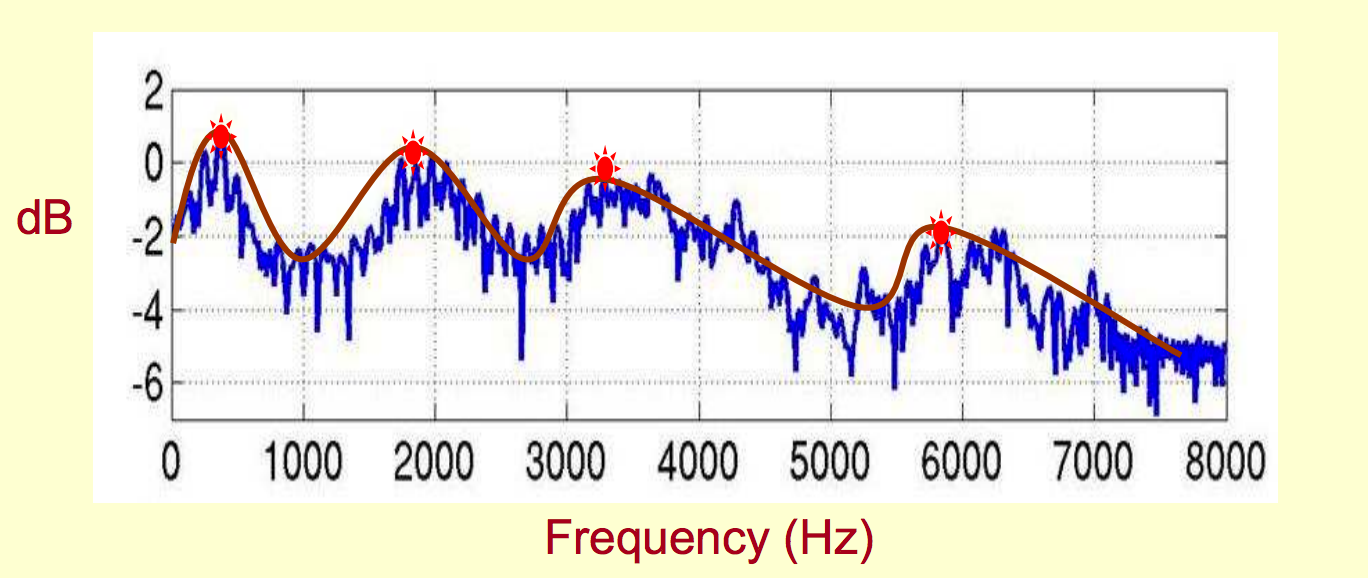
\includegraphics[width=\textwidth]{source//images/posts/spectral-envelope.png}\caption{Spectral Envelope}\label{fig:spectral-envelope}\end{figure}

Cepstral analysis is a way to separate the envelope from the spectrum.
As shown in the figure (\autoref{fig:cepstrum}), if we consider the log
spectrum as waveform, the frequency(quefrency) of spectral envelope is
low, while that of spectral details is high. So we can filter the low
frequency region to get envelope.

\begin{figure}[h]\centering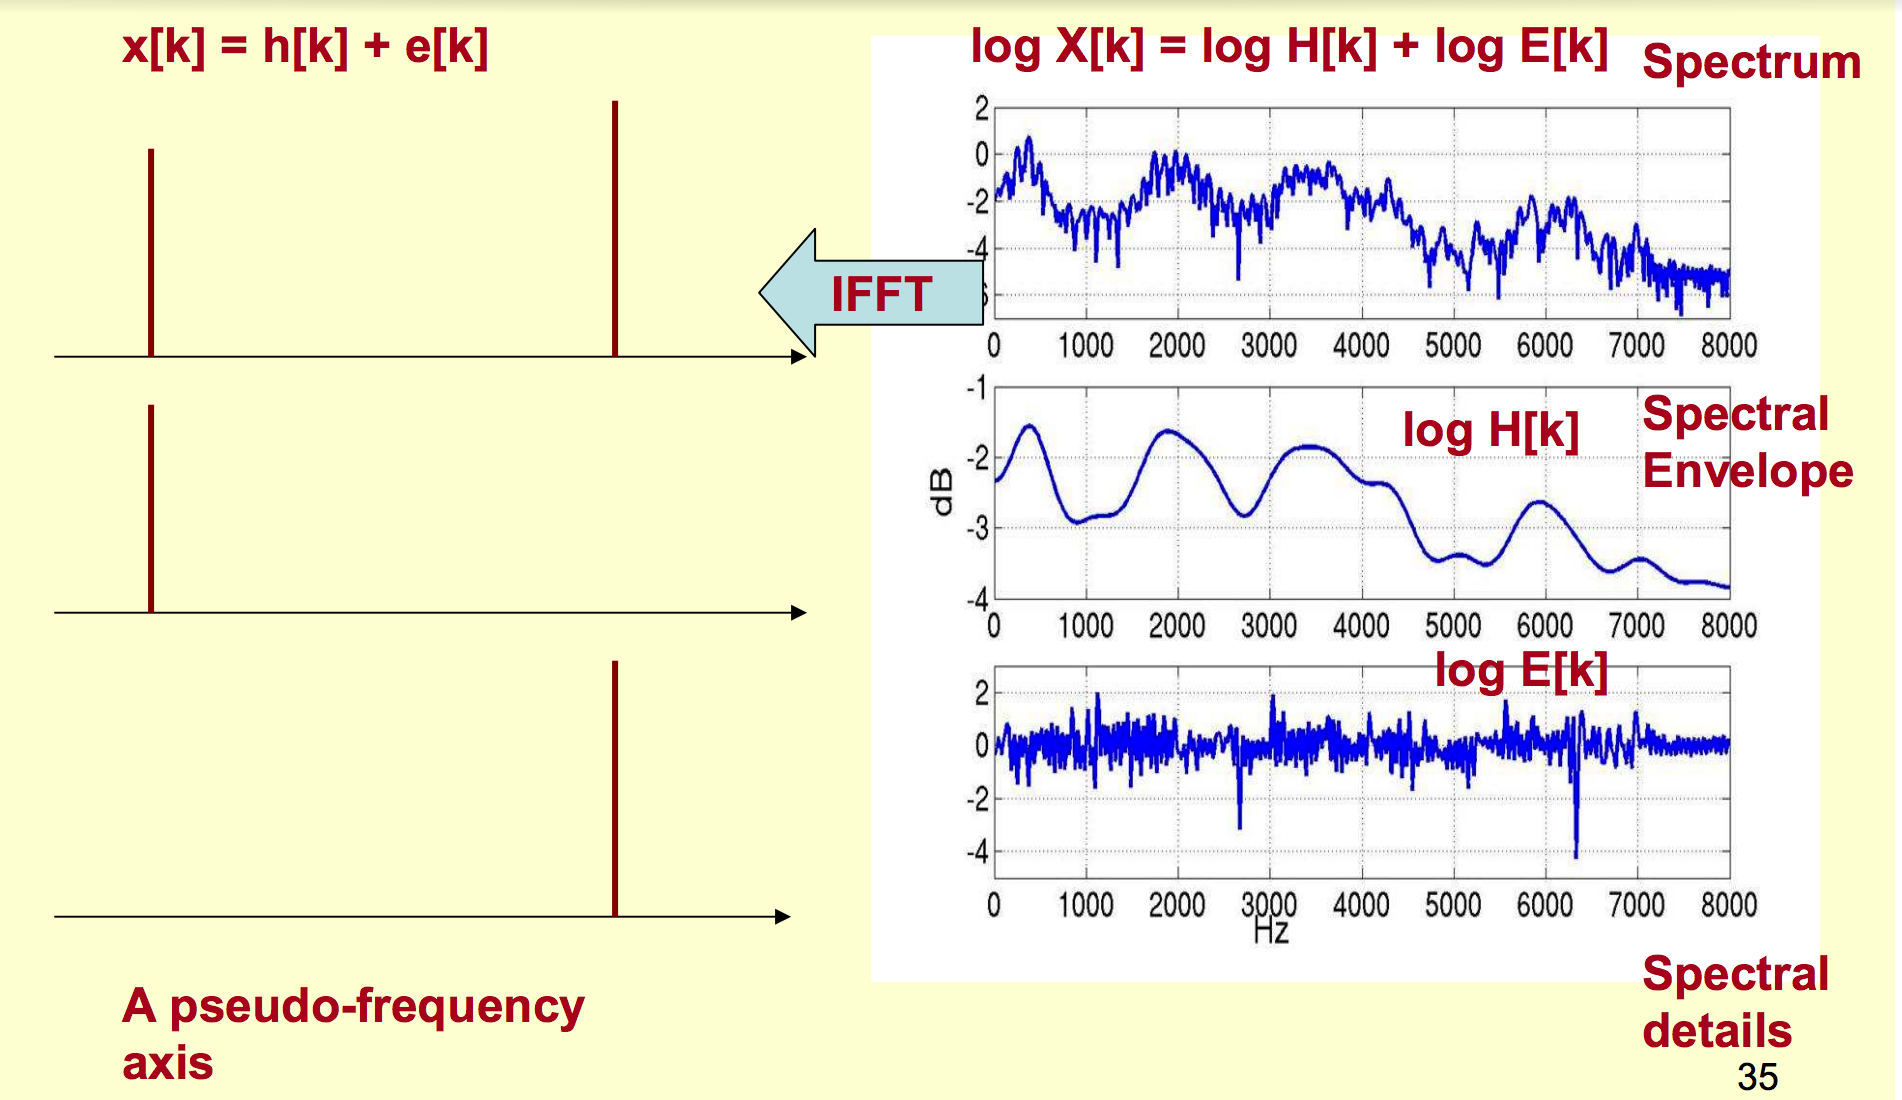
\includegraphics[width=\textwidth]{source//images/posts/cepstrum.png}\caption{Cepstrum}\label{fig:cepstrum}\end{figure}

Mathematically, let \(E[k]\) denotes spectral details(the periodic
excitation), \(H[k]\) denotes spectral envelope(vocal tract) and
\(X[k]\) denotes the spectrum of observed signal, then

\[
X[k] = E[k]H[k]
\]

\[
|X[k]|=|E[k]|\,|H[k]|
\]

Taking Log on both sides

\[
\log|X[k]|=\log|E[k]|+\log|H[k]|
\]

Taking inverseFFT on both sides

\[
x[k]=e[k]+h[k]
\]

Now the signal are separated with a simple addition. This procedure is
called de-convolution, more details can be found in
\href{http://www.speech.cs.cmu.edu/11-492/slides/03_mfcc.pdf}{this
slides}.

\section{Mel-Frequency Analysis}\label{mel-frequency-analysis}

The Mel scale relates perceived frequency, or pitch, of a pure tone to
its actual measured frequency. Humans are much better at discerning
small changes in pitch at low frequencies than they are at high
frequencies. Incorporating this scale makes our features match more
closely what humans hear.

This figure (\autoref{fig:mel}) shows the Mel-scale function. we can see
that Mel-scale gives more weight to low frequency regions. The values is
came from human perception experiments.

\begin{figure}[h]\centering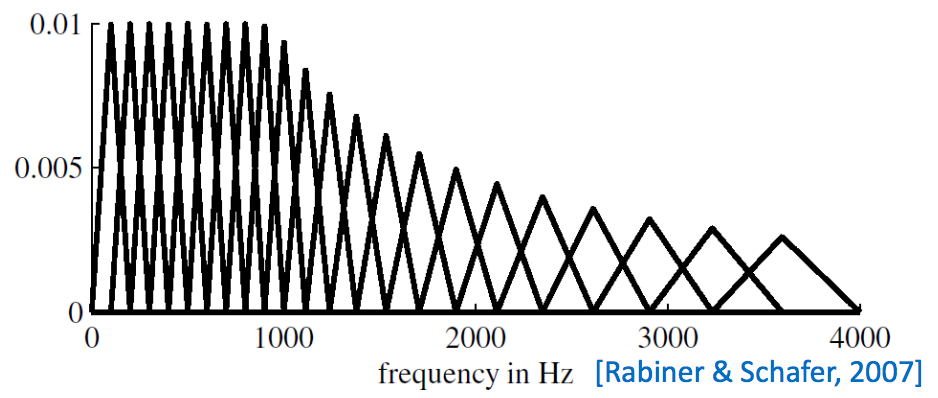
\includegraphics[width=\textwidth]{source//images/posts/mel.png}\caption{Mel scale}\label{fig:mel}\end{figure}

\section{implemntation}\label{implemntation}

To warp up, the complete recipe for extracting MFCC is,

\begin{enumerate}
\def\labelenumi{\arabic{enumi}.}
\itemsep1pt\parskip0pt\parsep0pt
\item
  Frame the signal into short frames.
\item
  For each frame calculate the power spectrum.
\item
  Apply the mel filterbank to the power spectra, sum the energy in each
  filter.
\item
  Take the logarithm of all filterbank energies.
\item
  Take the DCT of the log filterbank energies.
\item
  Keep DCT coefficients 2-13, discard the rest.
\end{enumerate}

\href{http://www.practicalcryptography.com/miscellaneous/machine-learning/guide-mel-frequency-cepstral-coefficients-mfccs/}{this
link} is a nice tutorial with python code.

\bibliographystyle{unsrt}

\bibliography{source/assets/printables/references}

\end{document}
